\section{Introduction}
Generative models are increasingly asked to produce objects whose admissible values form a curved or constrained space. Geographic locations lie on a sphere; torsion angles are periodic; covariance matrices must remain positive definite. An ambient Euclidean model can place probability outside the domain, and a final projection can distort the learned distribution. A useful construction should therefore address two distinct questions: how the output is constrained, and how the training objective uses the geometry of the data.

Riemannian Flow Matching (RFM) learns a time-dependent tangent vector field and generates samples by integrating that field \citep{chen2024general}. Its geometric interpolation is convenient when exponential and logarithm maps have closed forms. However, a simulation-free training target does not make inference one-step: sampling a continuous normalizing flow still requires repeated evaluations of its learned field. Midpoint Generative Models (MGM) instead train a static generator using a distribution discrepancy constructed from symmetrized interpolation fields \citep{shlenskii2026midpoint}. This suggests a complementary use of geometric interpolation: a training signal for a direct manifold-valued generator.

We develop this construction through reversible paths and tangent conditional expectations. Independent generated and data endpoints define a curve on the manifold. A hidden random flip selects a point at either time $t$ or $1-t$, while retaining the forward path velocity as the regression target. When endpoint laws agree, endpoint exchange preserves the observed point and reverses its tangent target. A critic that does not see the flip must therefore predict zero. The squared norm of its population optimum defines our geometric midpoint discrepancy.

Cancellation alone would be insufficient: different distributions could conceivably produce the same zero field. Our main result resolves this issue for the time-integrated construction. Integrating the actual path velocity against a Lipschitz test function recovers the difference between its endpoint expectations. This gives a Wasserstein-1 lower bound and hence definiteness on a general complete Riemannian manifold, without requiring densities or a global coordinate chart. Reversibility calibrates the discrepancy on equal distributions; the path derivative supplies the converse.

\begin{figure*}[t]
\centering
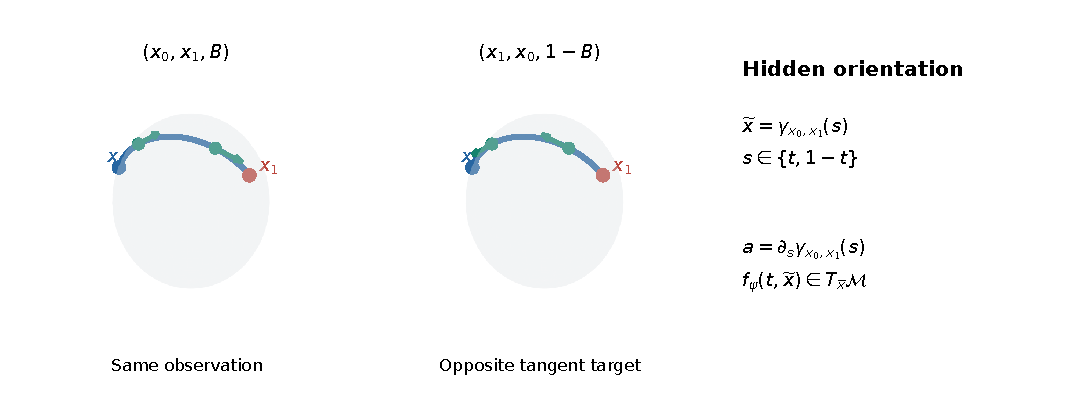
\includegraphics[width=\textwidth]{figures/method_symmetry.pdf}
\caption{\textbf{Geometric midpoint symmetry.} Two potential observations at $t$ and $1-t$ are shown on a sphere geodesic. Swapping endpoints and complementing the hidden flip preserves the selected point and reverses its tangent target. The critic sees $(t,\widetilde x)$, but not the flip or endpoints. These are schematic geometric curves, not experimental samples. At inference, only the constrained generator is used.}
\label{fig:symmetry}
\end{figure*}

Our contribution has three parts. First, we give an intrinsic, time-integrated midpoint discrepancy with a quantitative distributional guarantee and tangent-fiber variational representation. Second, we derive the corresponding one-step generator algorithm and specify its geometric and differentiation requirements. Third, we examine practical learning through initialization/objective controls, completed cells of a modern one-step comparison, and a two-object rigid-grasp pilot. The empirical record does not establish competitive superiority: the modern sweep is incomplete and geometric validity is not physical grasp success. The mesh study uses a projected surrogate rather than an exact spectral path.

\section{Background and Related Work}
\paragraph{Geometric flows and one-step maps.}
Flow Matching regresses a conditional path velocity rather than differentiating a likelihood through a learned ODE \citep{lipman2023flow}; stochastic interpolants provide a broader path-based viewpoint \citep{albergo2023building}. RFM and Riemannian score-based models incorporate manifold geometry into their objectives \citep{debortoli2022riemannian,chen2024general}. Consistency and flow-map approaches already provide one- or few-step manifold generation \citep{cheng2025rcm,davis2026gfm,woo2026rmf,zhong2026rmf}. We do not claim that one-step manifold generation is new. Our specific object is a hidden-flip conditional tangent-moment discrepancy and its variational training rule.

\paragraph{Midpoint and distributional objectives.}
MGM supplies midpoint cancellation and a variational quadratic critic in Euclidean space \citep{shlenskii2026midpoint}; Zero-Flow Encoders also study a zero-field criterion \citep{wang2026zeroflow}. MeanFlow learns average velocities \citep{geng2025mean}, while Drifting Models evolve a generator's output distribution during training \citep{deng2026drifting}. Kernel-Gradient Drifting Models extend kernel-induced fields to manifolds \citep{estebancasadevall2026kgdm}. Our tangent \emph{velocity} target requires its own argument: generalized stochastic MGM can use an endpoint chord, which is not the derivative of a noisy interpolant.

\paragraph{Wasserstein gradient flows.}
These flows decrease an energy on probability measures using optimal transport geometry \citep{jordan1998variational,ambrosio2008gradient}. Kernel discrepancies also admit such dynamics \citep{arbel2019maximum}. Recent one-step work includes W-Flow \citep{han2026wflow}, the Wasserstein interpretation of drifting \citep{gretton2026wasserstein}, RW-Flow on compact manifolds \citep{nurgulan2026rwflow}, and Riemannian Wasserstein gradient-flow models \citep{li2026rwgf}. The existence of these intrinsic one-step methods makes the choice of discrepancy, assumptions for identifiability, and practical objective the relevant comparison. Our theorem does not require a nondegenerate smoothing kernel, but does require full time coverage and true finite-energy path velocities. We distinguish the Riemannian metric on data from a Wasserstein metric on distributions; \cref{sec:wgf} explains why ordinary generator SGD is not automatically the latter's gradient flow.
